\subsection{M.PC.12 - Efficacia delle contromisure nei rischi}
\begin{figure}[H]
    \centering
    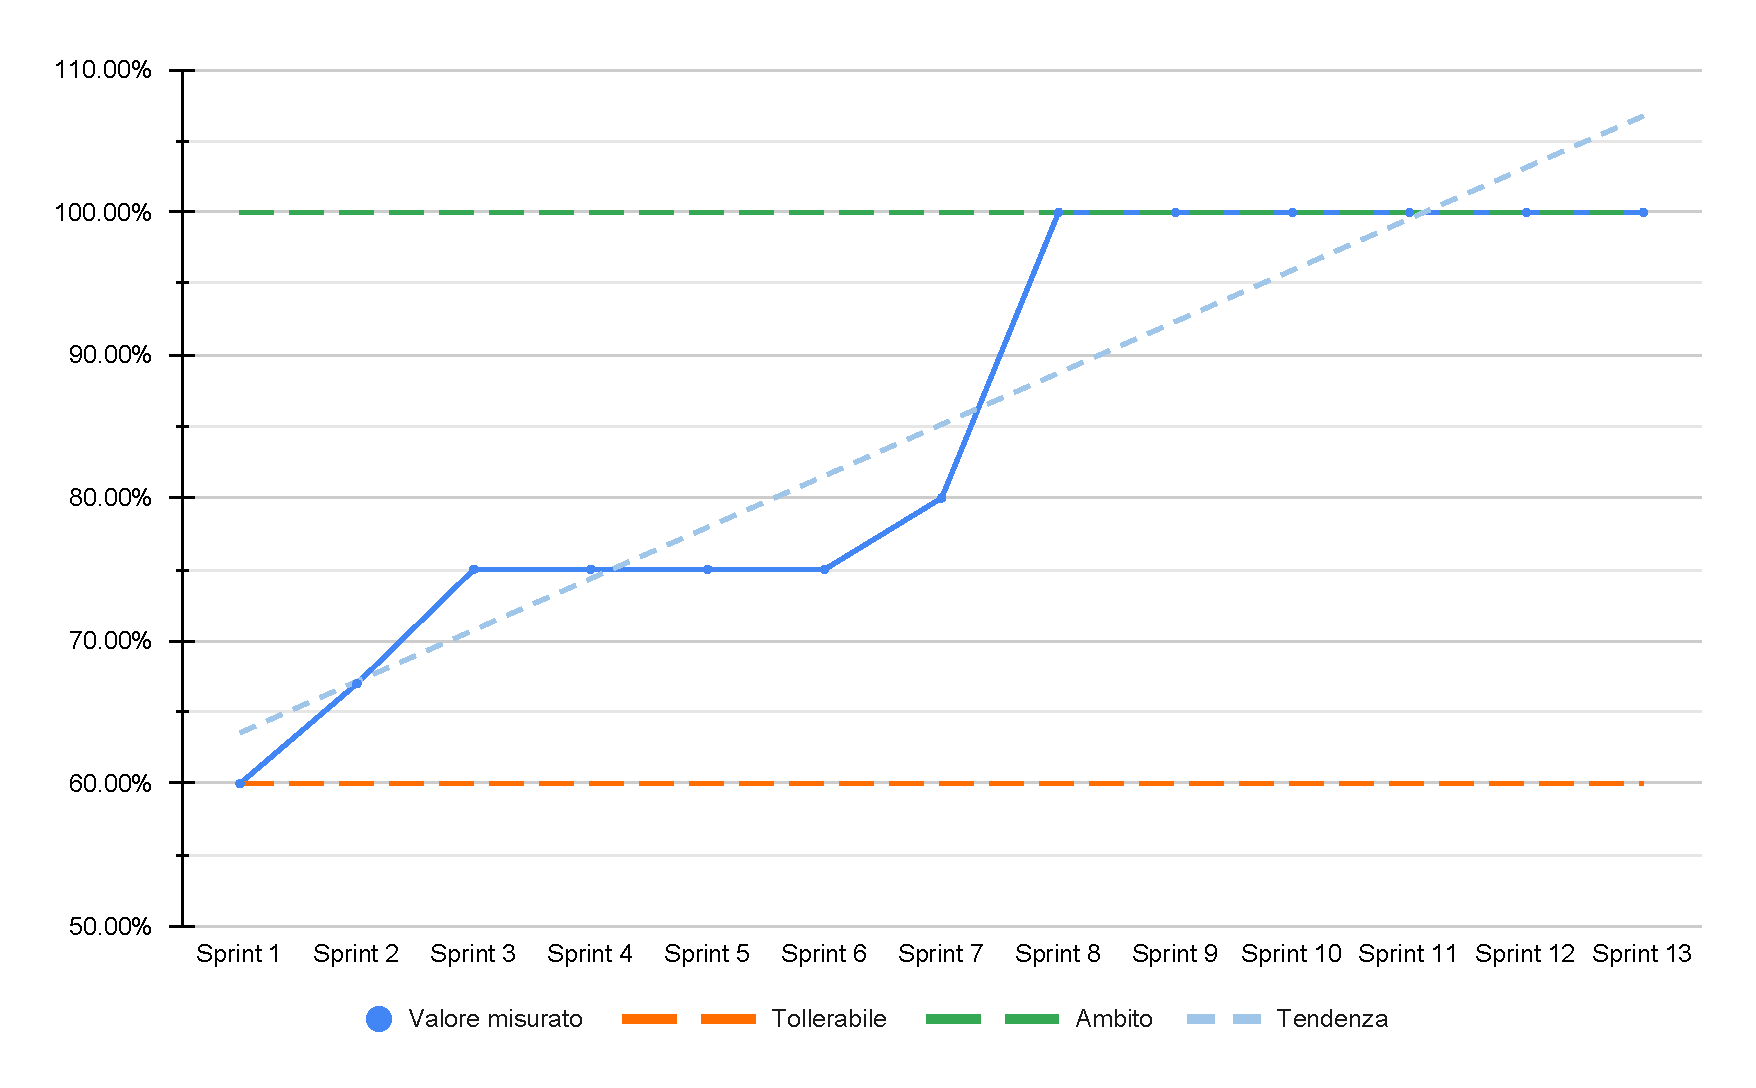
\includegraphics[width=\textwidth]{assets/efficacia_contromisure.pdf}
    \caption{M.PC.12 - Efficacia delle contromisure nei rischi}
\end{figure}

\par L'andamento dell'efficacia delle contromisure descrive un percorso di crescita da una fase iniziale di adattamento e apprendimento a una fase successiva di miglioramento continuo. Nei primi \glossario{sprint}, le contromisure applicate non risultavano sufficienti per garantire una puntuale e completa gestione dei rischi, evidenziando l’insperienza dell'analisi preliminare. A partire dal terzo sprint, il team ha sperimentato nuove strategie e procedure mirate ad affrontare e mitigare le difficoltà operative. Per ciascun rischio identificato, sono state introdotte almeno due contromisure, in modo tale da disporre dei cosiddetti fallback (opzioni di emergenza da adottare quando la soluzione primaria fallisce). Con l'accumulo di esperienza e l’introduzione di contromisure più specifiche, l'andamento dell'efficacia delle contromisure ha mostrato segnali di miglioramento. Un ulteriore problema rilevato dal team riguardava l’applicazione tardiva delle contromisure. Pertanto, sono state adottate nuove strategie di rilevamento, al fine di identificare e gestire i rischi con maggior tempestività. Queste strategie includono best practices e tecnologie applicate grazie ai feedback provenienti dall'esperienza pratica e dall’osservazione diretta. L’andamento del grafico testimonia la validità delle soluzioni applicate dal gruppo. Dopo un periodo iniziale di adattamento, infatti, l'impatto dei rischi è diminuito progressivamente. 
